\lstinputlisting[language=bash,basicstyle=\small]{python_codes/fieldstone_81/keywords.ascii}

\begin{center}
Code at \url{https://github.com/cedrict/fieldstone/tree/master/python_codes/fieldstone_81}
\end{center}

\par\noindent\rule{\textwidth}{0.4pt}
%%%%%%%%%%%%%%%%%%%%%%%%%%%%%%%%%%%%%%%%%%%%%%%%%%%%%%%%%%%%%%%%%%%%%%%%%%%%%%%%%%%%%%%%%%%%%%

This element is presented in Fortin (1981) \cite{fort81}. It is also mentioned in Dhatt \& Hubert (1986) \cite{dhhu86} and called 'H8N' and 
proved to be LBB-stable in the appendix.

\begin{center}
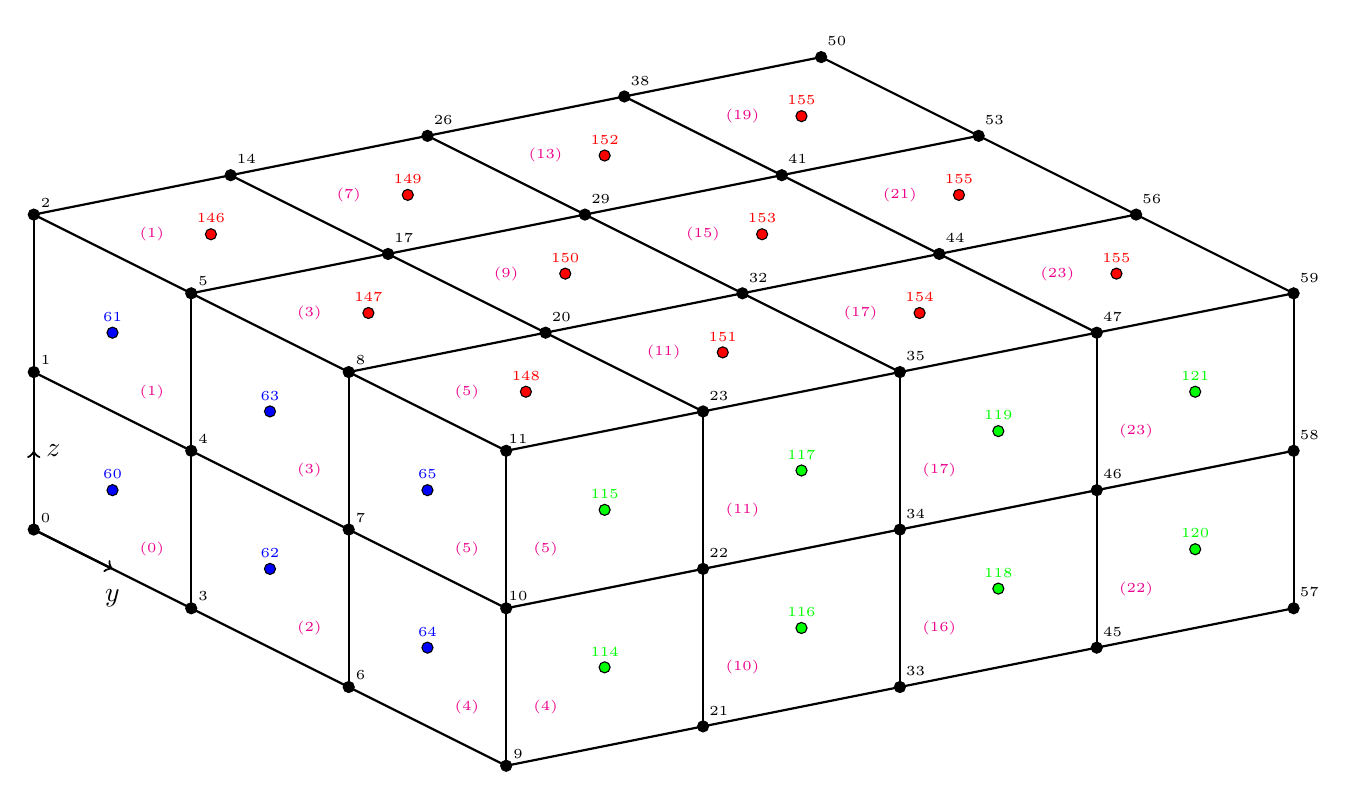
\begin{tikzpicture}
%\draw[fill=gray!23,gray!23](0,0) rectangle (16,9);
%\draw[step=0.5cm,gray,very thin] (0,0) grid (16,9); %background grid

\draw[thick] (0,3) -- (6,0) ;
\draw[thick] (0,5) -- (6,2) ;
\draw[thick] (0,7) -- (6,4) ;

\draw[thick] (2.5,7.5) -- (8.5,4.5) ;
\draw[thick] (5,8) -- (11,5) ;
\draw[thick] (7.5,8.5) -- (13.5,5.5) ;
\draw[thick] (10,9) -- (16,6) ;

\draw[thick] (0,3) -- (0,7) ;
\draw[thick] (2,2) -- (2,6) ;
\draw[thick] (4,1) -- (4,5) ;
\draw[thick] (6,0) -- (6,4) ;

\draw[thick] (0,7) -- (10,9) ;
\draw[thick] (2,6) -- (12,8) ;
\draw[thick] (4,5) -- (14,7) ;
\draw[thick] (6,4) -- (16,6) ;

\draw[thick] (6,2) -- (16,4) ;
\draw[thick] (6,0) -- (16,2) ;

\draw[thick] (8.5,0.5) -- (8.5,4.5) ;
\draw[thick] (11,1) -- (11,5) ;
\draw[thick] (13.5,1.5) -- (13.5,5.5) ;
\draw[thick] (16,2) -- (16,6) ;

\draw[black,fill=black] (0,3)   circle (2pt); \node[] at (0.15,3.15) {\tiny 0};
\draw[black,fill=black] (0,5)   circle (2pt); \node[] at (0.15,5.15) {\tiny 1};
\draw[black,fill=black] (0,7)   circle (2pt); \node[] at (0.15,7.15) {\tiny 2};

\draw[black,fill=black] (2,2)   circle (2pt); \node[] at (2.15,2.15) {\tiny 3};
\draw[black,fill=black] (2,4)   circle (2pt); \node[] at (2.15,4.15) {\tiny 4};
\draw[black,fill=black] (2,6)   circle (2pt); \node[] at (2.15,6.15) {\tiny 5};

\draw[black,fill=black] (4,1)   circle (2pt); \node[] at (4.15,1.15) {\tiny 6};
\draw[black,fill=black] (4,3)   circle (2pt); \node[] at (4.15,3.15) {\tiny 7};
\draw[black,fill=black] (4,5)   circle (2pt); \node[] at (4.15,5.15) {\tiny 8};

\draw[black,fill=black] (6,0)   circle (2pt); \node[] at (6.15,0.15) {\tiny 9};
\draw[black,fill=black] (6,2)   circle (2pt); \node[] at (6.15,2.15) {\tiny 10};
\draw[black,fill=black] (6,4)   circle (2pt); \node[] at (6.15,4.15) {\tiny 11};

\draw[black,fill=black] (8.5,0.5)   circle (2pt);  \node[] at (8.7,0.7) {\tiny 21};
\draw[black,fill=black] (8.5,2.5)   circle (2pt);  \node[] at (8.7,2.7) {\tiny 22};
\draw[black,fill=black] (8.5,4.5)   circle (2pt);  \node[] at (8.7,4.7) {\tiny 23};

\draw[black,fill=black] (11,1)   circle (2pt); \node[] at (11.2,1.2) {\tiny 33};
\draw[black,fill=black] (11,3)   circle (2pt); \node[] at (11.2,3.2) {\tiny 34};
\draw[black,fill=black] (11,5)   circle (2pt); \node[] at (11.2,5.2) {\tiny 35};

\draw[black,fill=black] (13.5,1.5)   circle (2pt); \node[] at (13.7,1.7) {\tiny 45};
\draw[black,fill=black] (13.5,3.5)   circle (2pt); \node[] at (13.7,3.7) {\tiny 46};
\draw[black,fill=black] (13.5,5.5)   circle (2pt); \node[] at (13.7,5.7) {\tiny 47};

\draw[black,fill=black] (16,2)   circle (2pt); \node[] at (16.2,2.2) {\tiny 57};
\draw[black,fill=black] (16,4)   circle (2pt); \node[] at (16.2,4.2) {\tiny 58};
\draw[black,fill=black] (16,6)   circle (2pt); \node[] at (16.2,6.2) {\tiny 59};

\draw[black,fill=black] (6.5,5.5)  circle (2pt); \node[] at (6.7,5.7) {\tiny 20};
\draw[black,fill=black] (9,6)      circle (2pt); \node[] at (9.2,6.2) {\tiny 32};
\draw[black,fill=black] (11.5,6.5) circle (2pt); \node[] at (11.7,6.7) {\tiny 44};
\draw[black,fill=black] (14,7)     circle (2pt); \node[] at (14.2,7.2) {\tiny 56};

\draw[black,fill=black] (4.5,6.5) circle (2pt); \node[] at (4.7,6.7) {\tiny 17};
\draw[black,fill=black] (7,7)     circle (2pt); \node[] at (7.2,7.2) {\tiny 29};
\draw[black,fill=black] (9.5,7.5) circle (2pt); \node[] at (9.7,7.7) {\tiny 41};
\draw[black,fill=black] (12,8)    circle (2pt); \node[] at (12.2,8.2) {\tiny 53};

\draw[black,fill=black] (2.5,7.5) circle (2pt); \node[] at (2.7,7.7) {\tiny 14};
\draw[black,fill=black] (5,8)     circle (2pt); \node[] at (5.2,8.2) {\tiny 26};
\draw[black,fill=black] (7.5,8.5) circle (2pt); \node[] at (7.7,8.7) {\tiny 38};
\draw[black,fill=black] (10,9)    circle (2pt); \node[] at (10.2,9.2) {\tiny 50};

\draw[black,fill=blue] (1,3.5) circle (2pt); \node[] at (1,3.7) {\tiny \color{blue} 60};
\draw[black,fill=blue] (1,5.5) circle (2pt); \node[] at (1,5.7) {\tiny \color{blue} 61};
\draw[black,fill=blue] (3,2.5) circle (2pt); \node[] at (3,2.7) {\tiny \color{blue} 62};
\draw[black,fill=blue] (3,4.5) circle (2pt); \node[] at (3,4.7) {\tiny \color{blue} 63};
\draw[black,fill=blue] (5,1.5) circle (2pt); \node[] at (5,1.7) {\tiny \color{blue} 64};
\draw[black,fill=blue] (5,3.5) circle (2pt); \node[] at (5,3.7) {\tiny \color{blue} 65};

\draw[black,fill=green](7.25,1.25) circle (2pt);\node[] at (7.25,1.45){\tiny\color{green}114};
\draw[black,fill=green](7.25,3.25) circle (2pt);\node[] at (7.25,3.45){\tiny\color{green}115};
\draw[black,fill=green](9.75,1.75) circle (2pt);\node[] at (9.75,1.95){\tiny\color{green}116};
\draw[black,fill=green](9.75,3.75) circle (2pt);\node[] at (9.75,3.95){\tiny\color{green}117};
\draw[black,fill=green](12.25,2.25) circle (2pt);\node[] at (12.25,2.45){\tiny\color{green}118};
\draw[black,fill=green](12.25,4.25) circle (2pt);\node[] at (12.25,4.45){\tiny\color{green}119};
\draw[black,fill=green](14.75,2.75) circle (2pt);\node[] at (14.75,2.95){\tiny\color{green}120};
\draw[black,fill=green](14.75,4.75) circle (2pt);\node[] at (14.75,4.95){\tiny\color{green}121};

\draw[black,fill=red] (2.25,6.75) circle (2pt); \node[] at (2.25,6.95) {\tiny \color{red} 146};
\draw[black,fill=red] (4.25,5.75) circle (2pt); \node[] at (4.25,5.95) {\tiny \color{red} 147};
\draw[black,fill=red] (6.25,4.75) circle (2pt); \node[] at (6.25,4.95) {\tiny \color{red} 148};

\draw[black,fill=red] (4.75,7.25) circle (2pt); \node[] at (4.75,7.45) {\tiny \color{red} 149};
\draw[black,fill=red] (6.75,6.25) circle (2pt); \node[] at (6.75,6.45) {\tiny \color{red} 150};
\draw[black,fill=red] (8.75,5.25) circle (2pt); \node[] at (8.75,5.45) {\tiny \color{red} 151};

\draw[black,fill=red] (7.25,7.75) circle (2pt); \node[] at (7.25,7.95) {\tiny \color{red} 152};
\draw[black,fill=red] (9.25,6.75) circle (2pt); \node[] at (9.25,6.95) {\tiny \color{red} 153};
\draw[black,fill=red] (11.25,5.75) circle (2pt); \node[] at (11.25,5.95) {\tiny \color{red} 154};

\draw[black,fill=red] (9.75,8.25) circle (2pt); \node[] at (9.75,8.45) {\tiny \color{red} 155};
\draw[black,fill=red] (11.75,7.25) circle (2pt); \node[] at (11.75,7.45) {\tiny \color{red} 155};
\draw[black,fill=red] (13.75,6.25) circle (2pt); \node[] at (13.75,6.45) {\tiny \color{red} 155};

\node[] at (1.5,2.75) {\tiny \color{magenta} (0)};
\node[] at (1.5,4.75) {\tiny \color{magenta} (1)};
\node[] at (3.5,1.75) {\tiny \color{magenta} (2)};
\node[] at (3.5,3.75) {\tiny \color{magenta} (3)};
\node[] at (5.5,0.75) {\tiny \color{magenta} (4)};
\node[] at (5.5,2.75) {\tiny \color{magenta} (5)};

\node[] at (6.5,0.75) {\tiny \color{magenta} (4)};
\node[] at (6.5,2.75) {\tiny \color{magenta} (5)};
\node[] at (9,1.25) {\tiny \color{magenta} (10)};
\node[] at (9,3.25) {\tiny \color{magenta} (11)};
\node[] at (11.5,1.75) {\tiny \color{magenta} (16)};
\node[] at (11.5,3.75) {\tiny \color{magenta} (17)};
\node[] at (14,2.25) {\tiny \color{magenta} (22)};
\node[] at (14,4.25) {\tiny \color{magenta} (23)};

\node[] at (5.5,4.75) {\tiny \color{magenta} (5)};
\node[] at (8,5.25) {\tiny \color{magenta} (11)};
\node[] at (10.5,5.75) {\tiny \color{magenta} (17)};
\node[] at (13,6.25) {\tiny \color{magenta} (23)};

\node[] at (3.5,5.75) {\tiny \color{magenta} (3)};
\node[] at (6,6.25) {\tiny \color{magenta} (9)};
\node[] at (8.5,6.75) {\tiny \color{magenta} (15)};
\node[] at (11,7.25) {\tiny \color{magenta} (21)};

\node[] at (1.5,6.75) {\tiny \color{magenta} (1)};
\node[] at (4,7.25) {\tiny \color{magenta} (7)};
\node[] at (6.5,7.75) {\tiny \color{magenta} (13)};
\node[] at (9,8.25) {\tiny \color{magenta} (19)};

\draw[thick,->] (0,3) -- (0,4); %x
\draw[thick,->] (0,3) -- (1,2.5); %y
\node[] at (1,2.125) {$y$};
\node[] at (0.25,4) {$z$};

\end{tikzpicture}\\
{\captionfont Example of a simple 4x3x2 mesh. Additional face dofs are indicated in colour.}
\end{center}

Each element has 
\begin{itemize}
\item 8+2 u dofs
\item 8+2 v dofs
\item 8+2 w dofs
\end{itemize}

Setting nelx=4, nely=3 and nelz=2, we can print the three connectivity arrays\footnote{it is the simplest way I found to account 
for the additional dofs in the three dimensions: a connectivity array per dimension.}:

\begin{itemize}
\item iconu:

\begin{verbatim}
0 [ 0 12 15  3  1 13 16  4 60 66]
1 [ 1 13 16  4  2 14 17  5 61 67]
2 [ 3 15 18  6  4 16 19  7 62 68]
3 [ 4 16 19  7  5 17 20  8 63 69]
4 [ 6 18 21  9  7 19 22 10 64 70]
5 [ 7 19 22 10  8 20 23 11 65 71]
6 [12 24 27 15 13 25 28 16 66 72]
7 [13 25 28 16 14 26 29 17 67 73]
8 [15 27 30 18 16 28 31 19 68 74]
9 [16 28 31 19 17 29 32 20 69 75]
10 [18 30 33 21 19 31 34 22 70 76]
11 [19 31 34 22 20 32 35 23 71 77]
12 [24 36 39 27 25 37 40 28 72 78]
13 [25 37 40 28 26 38 41 29 73 79]
14 [27 39 42 30 28 40 43 31 74 80]
15 [28 40 43 31 29 41 44 32 75 81]
16 [30 42 45 33 31 43 46 34 76 82]
17 [31 43 46 34 32 44 47 35 77 83]
18 [36 48 51 39 37 49 52 40 78 84]
19 [37 49 52 40 38 50 53 41 79 85]
20 [39 51 54 42 40 52 55 43 80 86]
21 [40 52 55 43 41 53 56 44 81 87]
22 [42 54 57 45 43 55 58 46 82 88]
23 [43 55 58 46 44 56 59 47 83 89]
\end{verbatim}

\item iconv:
\begin{verbatim}
0 [ 0 12 15  3  1 13 16  4 90 98]
1 [ 1 13 16  4  2 14 17  5 91 99]
2 [  3  15  18   6   4  16  19   7  98 106]
3 [  4  16  19   7   5  17  20   8  99 107]
4 [  6  18  21   9   7  19  22  10 106 114]
5 [  7  19  22  10   8  20  23  11 107 115]
6 [ 12  24  27  15  13  25  28  16  92 100]
7 [ 13  25  28  16  14  26  29  17  93 101]
8 [ 15  27  30  18  16  28  31  19 100 108]
9 [ 16  28  31  19  17  29  32  20 101 109]
10 [ 18  30  33  21  19  31  34  22 108 116]
11 [ 19  31  34  22  20  32  35  23 109 117]
12 [ 24  36  39  27  25  37  40  28  94 102]
13 [ 25  37  40  28  26  38  41  29  95 103]
14 [ 27  39  42  30  28  40  43  31 102 110]
15 [ 28  40  43  31  29  41  44  32 103 111]
16 [ 30  42  45  33  31  43  46  34 110 118]
17 [ 31  43  46  34  32  44  47  35 111 119]
18 [ 36  48  51  39  37  49  52  40  96 104]
19 [ 37  49  52  40  38  50  53  41  97 105]
20 [ 39  51  54  42  40  52  55  43 104 112]
21 [ 40  52  55  43  41  53  56  44 105 113]
22 [ 42  54  57  45  43  55  58  46 112 120]
23 [ 43  55  58  46  44  56  59  47 113 121]
\end{verbatim}

\item iconw:
\begin{verbatim}
0 [  0  12  15   3   1  13  16   4 122 134]
1 [  1  13  16   4   2  14  17   5 134 146]
2 [  3  15  18   6   4  16  19   7 123 135]
3 [  4  16  19   7   5  17  20   8 135 147]
4 [  6  18  21   9   7  19  22  10 124 136]
5 [  7  19  22  10   8  20  23  11 136 148]
6 [ 12  24  27  15  13  25  28  16 125 137]
7 [ 13  25  28  16  14  26  29  17 137 149]
8 [ 15  27  30  18  16  28  31  19 126 138]
9 [ 16  28  31  19  17  29  32  20 138 150]
10 [ 18  30  33  21  19  31  34  22 127 139]
11 [ 19  31  34  22  20  32  35  23 139 151]
12 [ 24  36  39  27  25  37  40  28 128 140]
13 [ 25  37  40  28  26  38  41  29 140 152]
14 [ 27  39  42  30  28  40  43  31 129 141]
15 [ 28  40  43  31  29  41  44  32 141 153]
16 [ 30  42  45  33  31  43  46  34 130 142]
17 [ 31  43  46  34  32  44  47  35 142 154]
18 [ 36  48  51  39  37  49  52  40 131 143]
19 [ 37  49  52  40  38  50  53  41 143 155]
20 [ 39  51  54  42  40  52  55  43 132 144]
21 [ 40  52  55  43  41  53  56  44 144 156]
22 [ 42  54  57  45  43  55  58  46 133 145]
23 [ 43  55  58  46  44  56  59  47 145 157]
\end{verbatim}

\end{itemize}


\begin{center}
a)\includegraphics[width=5.6cm]{python_codes/fieldstone_81/results/matrix4}
b)\includegraphics[width=5.6cm]{python_codes/fieldstone_81/results/matrix8}
c)\includegraphics[width=5.6cm]{python_codes/fieldstone_81/results/matrix12}\\
d)\includegraphics[width=5.6cm]{python_codes/fieldstone_81/results/matrix16}
e)\includegraphics[width=5.6cm]{python_codes/fieldstone_81/results/matrix20}
f)\includegraphics[width=5.6cm]{python_codes/fieldstone_81/results/matrix24}\\
{\captionfont non-zero pattern of the assembled Stokes matrix for $8^3$ (a), 
$12^3$ (b), $16^3$ (c) and $20^3$ (d) meshes.}
\end{center}
This is bad news: a renumbering of the nodes/dofs would be beneficial so as to reduce the 
skyline of the matrix. 

%----------------------------------------------------
\subsection*{Manufactured solution ({\tt bench=1})}

This benchmark is presented in Section~\ref{mms3} and is called the 'Burstedde' benchmark in the ASPECT manual after 
the paper by Burstedde et al (2013) \cite{busa13}, although it originates in Dohrmann \& Bochev (2004) \cite{dobo04}. 
It was run with 3 different quadrature levels, $nq=2^3,3^3,4^3$. 
Unfortunately a resolution $24\times 24\times 24$ is the maximum which can be run as demonstrated 
by the following table:

\begin{center}
\begin{tabular}{llll}
\hline
resolution &Nfem           &build (s) &solve(s) \\
\hline\hline
12x12x12   &12207+1728     &21        &5.4\\
16x16x16   &27795+4096     &49        &40\\
20x20x20   &52983+8000     &98.3      &414\\
21x21x21   &61050+9261     &130       &753 \\
22x22x22   &69897+10648    &144       &1213\\
24x24x24   &90075+13824    &173       &2481\\
\hline
\end{tabular}
\end{center}
 
 
We recover a quadratic convergence for the velocity error and a linear convergence for the pressure error, 
similarly to the $Q_1\times P_0$ element:

\begin{center}
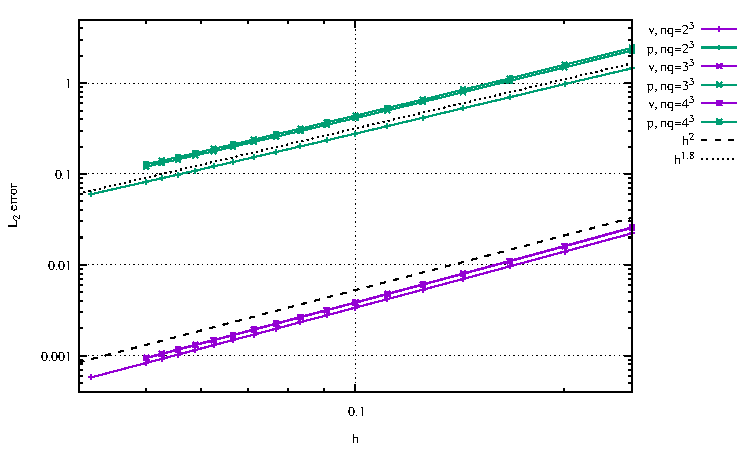
\includegraphics[width=10cm]{python_codes/fieldstone_81/results/bench1/conv.pdf}
\end{center}

It appears that a $2 \times 2\times 2$ is sufficient and yields the best results.

%----------------------------------------------------
\subsection*{Horizontal shear ({\tt bench=2})}

Gravity is set to zero so that density values are irrelevant. Viscosity is set to 1.
Velocity boundary conditions $\frac12-z,0,0$ are prescribed at the top and bottom, 
while the side boundaries are left free. We expect this same velocity field everywhere in the 
domain and given the pressure normalisation a zero pressure in the domain. 

\begin{center}
\includegraphics[width=8cm]{python_codes/fieldstone_81/results/bench2/vel}
\includegraphics[width=8cm]{python_codes/fieldstone_81/results/bench2/press}\\
\includegraphics[width=5cm]{python_codes/fieldstone_81/results/bench2/u}
\includegraphics[width=5cm]{python_codes/fieldstone_81/results/bench2/v}
\includegraphics[width=5cm]{python_codes/fieldstone_81/results/bench2/w}
\end{center}



%----------------------------------------------------
\subsection*{Stokes sphere benchmark ({\tt bench=3})}

It is described in Section~\ref{ss:stokes_sphere3D}. We here focus on the 'NS' case, i.e. no slip 
boundary conditions are prescribed on all six faces. Unfortunately the resolution is so limited 
that it is hard to really see a convergence in the results.

\begin{center}
\includegraphics[width=5.5cm]{python_codes/fieldstone_81/results/bench3/u}
\includegraphics[width=5.5cm]{python_codes/fieldstone_81/results/bench3/v}
\includegraphics[width=5.5cm]{python_codes/fieldstone_81/results/bench3/w}\\
\includegraphics[width=5.5cm]{python_codes/fieldstone_81/results/bench3/vel}
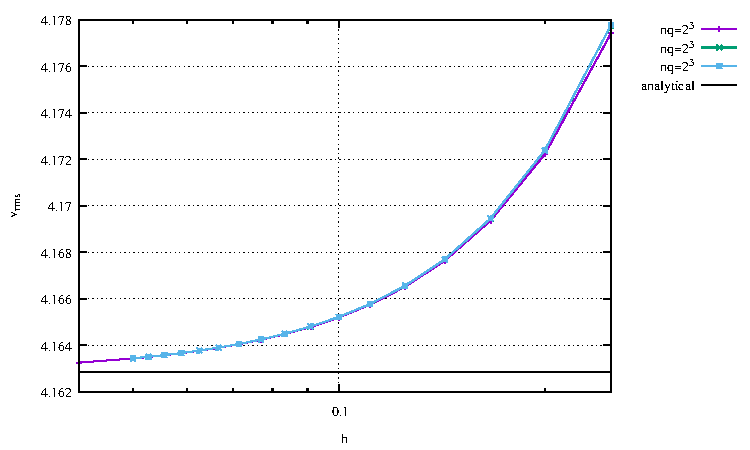
\includegraphics[width=5.5cm]{python_codes/fieldstone_81/results/bench3/vrms}
\includegraphics[width=5.5cm]{python_codes/fieldstone_81/results/bench3/press}
\end{center}




















 
